\documentclass[a4paper,10pt,fleqn,openright]{Quark}
% fleqn : left-justified equations
% openany : do not put blankpage if a new chapter start on a odd page
%% END Options


%%%%%%%%%%%%%%%%%%%%%%%%%%%%%
%% Footer

\renewcommand{\leftfootname}{University of ...}
\renewcommand{\middlefootname}{\it Dated: \today}
\renewcommand{\rightfootname}{\sc Name}


\definecolor{QuarkColor}{RGB}{21,81,149} % Main color

\definecolor{chaptergrey}{RGB}{21,81,149} % Chapter color


%%
%%%%%%%%%%%%%%%%%%%%%%%%%%%%%

%%%%%%%%%%%%%%%%%%%%%%%%%%%%%%%%%%%%%%%%%%%%%%%%%%%%%%%%%%%%%%%%%%
%% DOCUMENT 
%%%%%%%%%%%%%%%%%%%%%%%%%%%%%%%%%%%%%%%%%%%%%%%%%%%%%%%%%%%%%%%%%%

\begin{document}

%%%%%%%%%%%%%%%%%%%%%%%%%%%%%%%%%%%%%%%%%%%%%%%%%%%%%%%%%%%%%%%%%%
%% Cover 
%%%%%%%%%%%%%%%%%%%%%%%%%%%%%%%%%%%%%%%%%%%%%%%%%%%%%%%%%%%%%%%%%%

%\pagenumbering{roman}
\newgeometry{left=24.8mm,top=27.4mm,bottom=27.4mm,headheight=\baselineskip}
%\fancyhfoffset[LE,RO]{0mm}
%\fancyhfoffset[RO]{0mm}

% Title page
\thispagestyle{empty}


$~$

\vfill

\begin{large}
\noindent \textbf{The Quark template} \\
\noindent With examples \\
\end{large}

\noindent \textsc{D. Minenna} \\

\noindent Aix-Marseille University




\restoregeometry


%%%%%%%%%%%%%%%%%%%%%%%%%%%%%%%%%%%%%%%%%%%%%%%%%%%%%%%%%%%%%%%%%%
%% Licence 
%%%%%%%%%%%%%%%%%%%%%%%%%%%%%%%%%%%%%%%%%%%%%%%%%%%%%%%%%%%%%%%%%%

\newpage

\begin{adjustwidth}{0pt}{-\marginBiblio}

$~$

\vfill

\vspace{2cm}

\begin{center}
	\begin{minipage}[c]{0.25\linewidth}
		\raggedright
\includegraphics[height=35px]{Figs/by-nc-nd-eu.pdf}
	\end{minipage}\hfill
\end{center}

\noindent This document is put at disposal under the terms of the \href{https://creativecommons.org/licenses/by-nc-nd/4.0/}{Creative Commons Licence: Attribution - NonCommercial - NoDerivatives 4.0 International (CC BY-NC-ND 4.0)}. 

\end{adjustwidth}

%%%%%%%%%%%%%%%%%%%%%%%%%%%%%%%%%%%%%%%%%%%%%%%%%%%%%%%%%%%%%%%%%%
%% Abstract 
%%%%%%%%%%%%%%%%%%%%%%%%%%%%%%%%%%%%%%%%%%%%%%%%%%%%%%%%%%%%%%%%%%

\newpage

\begin{adjustwidth}{0pt}{-\marginBiblio}

%% Chapter Abstract. See abstract.txt in the TeX folder
\chapter*{Abstract}
\thispagestyle{fancy}
\addcontentsline{toc}{chapter}{\protect\numberline{}Abstract}%

This is the abstract.

Lorem ipsum dolor sit amet, consectetuer adipiscing elit. Ut purus elit, vestibulum ut, placerat ac, adipiscing
vitae, felis. Curabitur dictum gravida mauris. Nam arcu libero, nonummy eget, consectetuer id, vulputate a, magna. Donec vehicula augue eu neque. Pellentesque habitant morbi tristique senectus et netus et malesuada fames ac turpis egestas. Mauris ut leo. Cras viverra metus rhoncus sem. Nulla et lectus vestibulum urna fringilla ultrices. Phasellus eu tellus sit amet tortor gravida placerat. Integer sapien est, iaculis in, pretium quis, viverra ac, nunc. Praesent eget sem vel leo ultrices bibendum. Aenean faucibus. Morbi dolor nulla, malesuada eu, pulvinar at, mollis ac, nulla. Curabitur auctor semper nulla. Donec varius orci eget risus. Duis nibh mi, congue eu, accumsan eleifend, sagittis quis, diam. Duis eget orci sit amet orci dignissim rutrum.
Nam dui ligula, fringilla a, euismod sodales, sollicitudin vel, wisi. Morbi auctor lorem non justo. Nam lacus libero, pretium at, lobortis vitae, ultricies et, tellus. Donec aliquet, tortor sed accumsan bibendum, erat ligula aliquet magna, vitae ornare odio metus a mi. Morbi ac orci et nisl hendrerit mollis. Suspendisse ut massa. Cras nec ante. Pellentesque a nulla. Cum sociis natoque penatibus et magnis dis parturient montes, nascetur ridiculus mus. Aliquam tincidunt urna. Nulla ullamcorper vestibulum turpis. Pellentesque cursus luctus mauris.
Nulla malesuada porttitor diam. Donec felis erat, congue non, volutpat at, tincidunt tristique, libero. Vivamus viverra fermentum felis. Donec nonummy pellentesque ante. Phasellus adipiscing semper elit. Proin fermentum massa ac quam. Sed diam turpis, molestie vitae, placerat a, molestie nec, leo. Maecenas lacinia. Nam ipsum ligula, eleifend at, accumsan nec, suscipit a, ipsum. Morbi blandit ligula feugiat magna. Nunc eleifend consequat lorem. Sed lacinia nulla vitae enim. Pellentesque tincidunt purus vel magna. Integer non enim. Praesent euismod nunc eu purus. Donec bibendum quam in tellus. Nullam cursus pulvinar lectus. Donec et mi. Nam vulputate metus eu enim. Vestibulum pellentesque felis eu massa.

\end{adjustwidth}

%%%%%%%%%%%%%%%%%%%%%%%%%%%%%%%%%%%%%%%%%%%%%%%%%%%%%%%%%%%%%%%%%%
%% Thanks 
%%%%%%%%%%%%%%%%%%%%%%%%%%%%%%%%%%%%%%%%%%%%%%%%%%%%%%%%%%%%%%%%%%

\newpage

\begin{adjustwidth}{0pt}{-\marginBiblio}

% Chapter Thanks
% Add the chapter name in the header
\markboth{Thanks}{}

% Quote
\begin{savequote}[90mm]
On a dark desert highway \\
Cool wind in my hair \\
Warm smell of colitas \\
Rising up through the air
\qauthor{--- Eagles, \textit{Hotel California}, 1977}
\end{savequote}

\chapter*{Thanks} 
\thispagestyle{fancy}

% Add entry in the contents
\addcontentsline{toc}{chapter}{\protect\numberline{}Thanks}


%% From here you can write your chapter content


\lipsum[1-5] 

% table of contents
\addcontentsline{toc}{chapter}{\protect\numberline{}Contents}%
\thispagestyle{fancy}
\setcounter{tocdepth}{1}
\tableofcontents

\end{adjustwidth}


%%%%%%%%%%%%%%%%%%%%%%%%%%%%%%%%%%%%%%%%%%%%%%%%%%%%%%%%%%%%%%%%%%
%% BODY 
%%%%%%%%%%%%%%%%%%%%%%%%%%%%%%%%%%%%%%%%%%%%%%%%%%%%%%%%%%%%%%%%%%

% Begining of the body
\makeatletter
\renewcommand{\@makechapterhead}[1]{%
  \chapterheadstartvskip%
  {\size@chapter{\sectfont
    {  \begin{adjustwidth}{0pt}{-\marginBiblio}
     {\raggedleft\chapnumfont
      \ifnum \c@secnumdepth >\m@ne%
        \if@mainmatter\thechapter\else\phantom{\thechapter}%
      \fi\else\phantom{\thechapter}\fi
      \par\nobreak}%
      \end{adjustwidth}
      }
    { \begin{adjustwidth}{0pt}{-\marginBiblio}
    {\raggedleft\advance\leftmargin10em\interlinepenalty\@M #1\par}
    \end{adjustwidth} }}
  \nobreak\chapterheadendvskip}
  }%
\makeatother

% New part
\part{First part}	
\newpage
$~$
\newpage

\begin{savequote}[120mm]
Up ahead in the distance \\
I saw a shimmering light \\
My head grew heavy and my sight grew dim \\
I had to stop for the night
\qauthor{--- Eagles, \textit{Hotel California}, 1977}
\end{savequote}


\chapter{The Quark template}
\label{chapter1}
\thispagestyle{fancy}

\textit{Lorem ipsum dolor sit amet, consectetuer adipiscing elit. Ut purus elit, vestibulum ut, plac- erat ac, adipiscing vitae, felis. Curabitur dictum gravida mauris. Nam arcu libero, nonummy eget, consectetuer id, vulputate a, magna. Donec vehicula augue eu neque. Pellentesque habitant morbi tristique senectus et netus et malesuada fames ac turpis egestas. Mauris ut leo. Cras viverra metus rhoncus sem. Nulla et lectus vestibulum urna fringilla ultrices. Phasellus eu tellus sit amet tortor gravida placerat. Integer sapien est, iaculis in, pretium quis, viverra ac, nunc. Praesent eget sem vel leo ultrices bibendum. Aenean faucibus. Morbi dolor nulla, malesuada eu, pulvinar at, mollis ac, nulla. Curabitur auctor semper nulla. Donec varius orci eget risus. Duis nibh mi, congue eu, accumsan eleifend, sagittis quis, diam. Duis eget orci sit amet orci dignissim rutrum.}

%{\chapHeadFont

\paragraph{Paragraph 1}

Lorem ipsum dolor sit amet, consectetuer adipiscing elit. Ut purus elit, vestibulum ut, plac- erat ac, adipiscing vitae, felis. Curabitur dictum gravida mauris. Nam arcu libero, nonummy eget, consectetuer id, vulputate a, magna. Donec vehicula augue eu neque. Pellentesque habitant morbi tristique senectus et netus et malesuada fames ac turpis egestas. Mauris ut leo. Cras viverra metus rhoncus sem. Nulla et lectus vestibulum urna fringilla ultrices. Phasellus eu tellus sit amet tortor gravida placerat. Integer sapien est, iaculis in, pretium quis, viverra ac, nunc. Praesent eget sem vel leo ultrices bibendum. Aenean faucibus. Morbi dolor nulla, malesuada eu, pulvinar at, mollis ac, nulla. Curabitur auctor semper nulla. Donec varius orci eget risus. Duis nibh mi, congue eu, accumsan eleifend, sagittis quis, diam. Duis eget orci sit amet orci dignissim rutrum.



\section{Bibliography, citation and hyperlink}

\subsection{hyperlink}

Use the command \texttt{secref} to refer to sections such as the \secref{sectionA}. Use the command \texttt{secref} to refer to sections such as the \chapref{chapter1}. There also exists the commands \texttt{appref, remref, figref, tabref} for appendices, remarks, figures and tables.

\subsection{Citations}

Citations and notes are put in the margin. To place a note use the command  \texttt{notenum}\notenum{Here a note with \texttt{notenum}.} Citations in the margin use the command \texttt{citenote}\citenote{mou11}. For citations in the text, just use \texttt{cite} such as \cite{lan46}. Citenotes can have several citations\citenote{mou11,lan46,nic83,bon90} and one can place several citation on the same\citenote{nic83,bon90} line.\citenote{che10}

\begin{remark}[Margins]
Margin are on the right side of the document. There are no planned option to place the margin on the left.
\end{remark}

\subsection{Bibliography}

We use the package natbib. Add new references using
\begin{verbatim}
\bibitem[Name(year)]{id1}  ...
\bibitem[Name1 \and Name2(year)]{id2}  ...
\bibitem[Name \etal(year)]{id3} ...
\end{verbatim} 

\section{Figures, ...}

\subsection{Figures with caption on the right}

There are two commands to place figures with the caption on the right.
\begin{verbatim}
% Large figure:
\figBesideLeft{file.jpg}{label}{Text caption}

% Small figure:
\figSmallLeft{file.jpg}{label}{Text caption}

% Cite them with \figref{label}.
\end{verbatim}
An alternative, with the caption below and intruded in the margins
\begin{verbatim}
\begin{figure}
\captionsetup{margin={-12mm,-28.8mm}}
\centering
{\caption{ Text caption }\label{label}}
{\hspace{40mm} \includegraphics[width=1\textwidth]{file.jpg}}
\end{figure}
\end{verbatim}

\subsection{Full text}

One can remove the margin using the environment
\begin{verbatim}
\begin{adjustwidth}{-12mm}{-\marginAll}
...
\end{adjustwidth}
\end{verbatim}
such as for this long equation
\begin{adjustwidth}{-12mm}{-\marginAll}
 \begin{equation}
  P_{n,z} (t) 
 = \sum_{s \in \ZZ} \left( \frac{1}{2 \pi}\right)^2 \Re \left[ \int_{- \pi}^\pi  \int_{- \pi}^\pi  \sV^{s*}_{\beta_1}(t) \, \sI^{s}_{\beta_2}(t) \, \mathfrak{k}^s_{\beta_1, \beta_2}   \frac{1}{d} \mathrm{sinc}\left( \frac{d}{2} ( \beta_2 - \beta_1 )\right) \, \rme^{-\rmi n d( \beta_2 - \beta_1 )} \,  \rmd (\beta_1 d) \, \rmd (\beta_2 d) \right]  \, .
  \label{e.PnKinbeta}
\end{equation}
\end{adjustwidth}


\section{Warning}

The warning ``Marginpar on page \# moved" and the warning Badbox ``Overfull hbox (...) detected" can appear during the compilation.

\section{Section}

\section{Small sub-section}

Lorem ipsum dolor sit amet, consectetuer adipiscing elit. Ut purus elit, vestibulum ut, plac- erat ac, adipiscing vitae, felis. Curabitur dictum gravida mauris. Nam arcu libero, nonummy eget, consectetuer id, vulputate a, magna. Donec vehicula augue eu neque. Pellentesque habitant morbi tristique senectus et netus et malesuada fames ac turpis egestas. Mauris ut leo. Cras viverra metus rhoncus sem. Nulla et lectus vestibulum urna fringilla ultrices. Phasellus eu tellus sit amet tortor gravida placerat. Integer sapien est, iaculis in, pretium quis, viverra ac, nunc. Praesent eget sem vel leo ultrices bibendum. 
\begin{align} \label{Maxwell}
\rot \bfE_{\rm tot}(\bfr,t) = -  \mu_0 \frac{\partial \bfH}{\partial t}(\bfr,t)\, ,  \qquad \epsilon_0 \, \div \bfE_{\rm tot}(\bfr,t) = \rho(\bfr,t) \, , \nonumber\\
\rot \bfH(\bfr,t) =  \epsilon_0 \frac{\partial \bfE_{\rm tot}}{\partial t}(\bfr,t) + \bfJ (\bfr,t)\, ,  \quad \mu_0 \, \div \bfH(\bfr,t) = 0 \, , 
\end{align}
Aenean faucibus. Morbi dolor nulla, malesuada eu, pulvinar at, mollis ac, nulla. Curabitur auctor semper nulla. Donec varius orci eget risus. Duis nibh mi, congue eu, accumsan eleifend, sagittis quis, diam. Duis eget orci sit amet orci dignissim rutrum.

\begin{remark}[Lorem]
Lorem ipsum dolor sit amet, consectetuer adipiscing elit. Ut purus elit, vestibulum ut, plac- erat ac, adipiscing vitae, felis. Curabitur dictum gravida mauris. Nam arcu libero, nonummy eget, consectetuer id, vulputate a, magna. Donec vehicula augue eu neque. Pellentesque habitant morbi tristique senectus et netus et malesuada fames ac turpis egestas. 
\end{remark}


\figBesideLeft{Figs/Fig_cat_eyes_wavicules.pdf}{f:portraitPhase}{Lorem ipsum dolor sit amet, consectetuer adipiscing elit. Ut purus elit, vestibulum ut, plac- erat ac, adipiscing vitae, felis. Curabitur dictum gravida mauris.}%

Nam dui ligula, fringilla a, euismod sodales, sollicitudin vel, wisi. Morbi auctor lorem non justo. Nam lacus libero, pretium at, lobortis vitae, ultricies et, tellus. Donec aliquet, tortor sed accumsan bibendum, erat ligula aliquet magna, vitae ornare odio metus a mi. Morbi ac orci et nisl hendrerit mollis. Suspendisse ut massa. Cras nec ante. Pellentesque a nulla. Cum sociis natoque penatibus et magnis dis parturient montes, nascetur ridiculus mus. Aliquam tincidunt urna. Nulla ullamcorper vestibulum turpis. Pellentesque cursus luctus mauris.
Nulla malesuada porttitor diam. Donec felis erat, congue non, volutpat at, tincidunt tris- tique, libero. Vivamus viverra fermentum felis. Donec nonummy pellentesque ante. Phasel- lus adipiscing semper elit. Proin fermentum massa ac quam. Sed diam turpis, molestie vitae, placerat a, molestie nec, leo. Maecenas lacinia. Nam ipsum ligula, eleifend at, accumsan nec, suscipit a, ipsum. Morbi blandit ligula feugiat magna. Nunc eleifend consequat lorem. Sed lacinia nulla vitae enim. Pellentesque tincidunt purus vel magna. Integer non enim. Praesent euismod nunc eu purus. Donec bibendum quam in tellus. Nullam cursus pulvinar lectus. Donec et mi. Nam vulputate metus eu enim. Vestibulum pellentesque felis eu massa.

\begin{definition}[Lipsum]
Donec et mi. Nam vulputate metus eu enim. Vestibulum pellentesque felis eu massa.
\end{definition}

\figSmallLeft{Figs/tube_Helix.pdf}{f:TubeHelix}{Lorem ipsum dolor sit amet, consectetuer adipiscing elit. Ut purus elit, vestibulum ut, plac- erat ac, adipiscing vitae, felis. Curabitur dictum gravida mauris.}

\lipsum[4-7]

\begin{figure}
\captionsetup{margin={-12mm,-28.8mm}}
\centering
{\caption{
Lorem ipsum dolor sit amet, consectetuer adipiscing elit. Ut purus elit, vestibulum ut, plac- erat ac, adipiscing vitae, felis. Curabitur dictum gravida mauris. Nam arcu libero, nonummy eget, consectetuer id, vulputate a, magna. Donec vehicula augue eu neque. Pellentesque habitant morbi tristique senectus et netus et malesuada fames ac turpis egestas. Mauris ut leo. Cras viverra metus rhoncus sem. Nulla et lectus vestibulum urna fringilla ultrices. Phasellus eu tellus sit amet tortor gravida placerat. Integer sapien est, iaculis in, pretium quis, viverra ac, nunc. Praesent eget sem vel leo ultrices bibendum. Aenean faucibus. Morbi dolor nulla, malesuada eu, pulvinar at, mollis ac, nulla. Curabitur auctor semper nulla. Donec varius orci eget risus. Duis nibh mi, congue eu, accumsan eleifend, sagittis quis, diam. Duis eget orci sit amet orci dignissim rutrum.}\label{figure4}}
{\hspace{40mm} 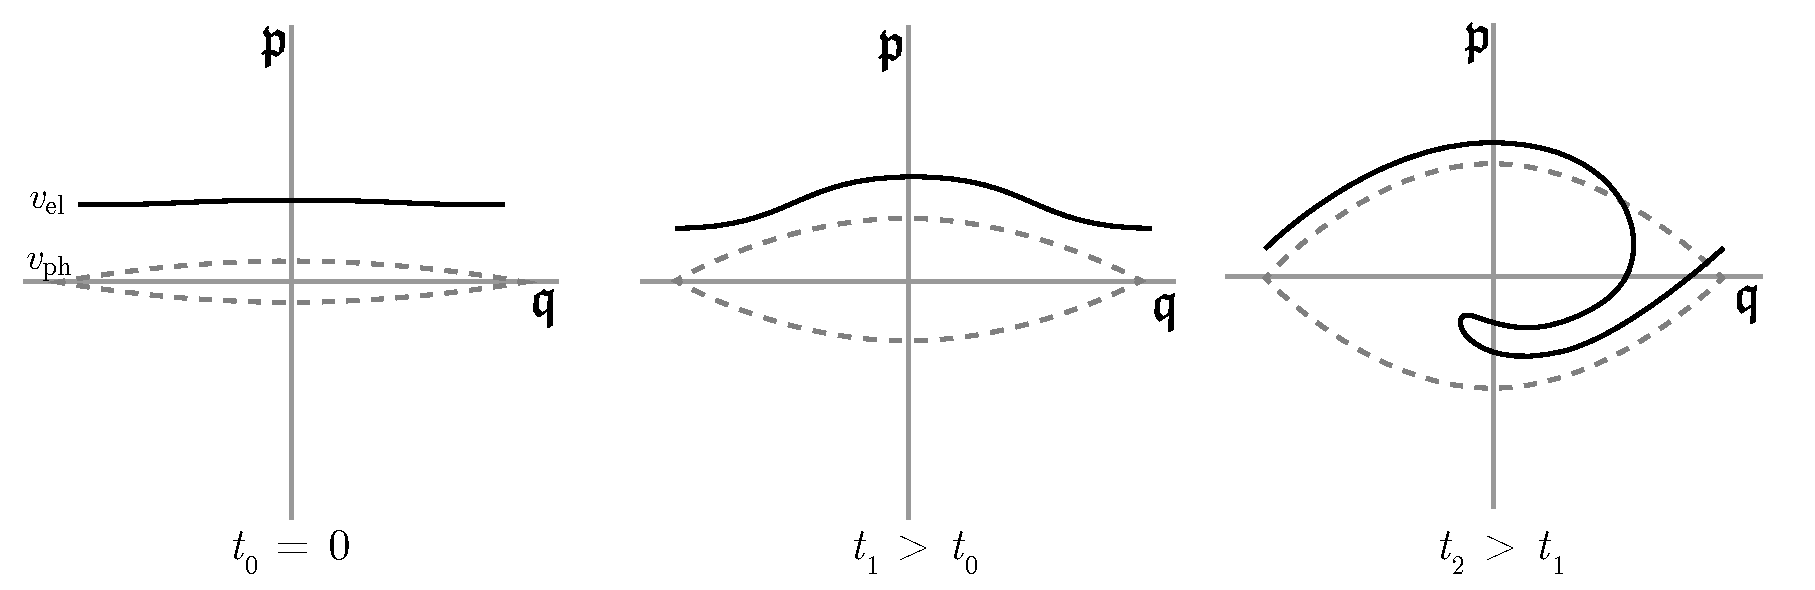
\includegraphics[width=1\textwidth]{Figs/Fig_cat_eyes_amplified.pdf}}
\end{figure}

\lipsum[4-7]

\begin{theorem}[Lipsum]
Donec et mi. Nam vulputate metus eu enim. Vestibulum pellentesque felis eu massa.
\end{theorem}

\begin{table}
\floatbox[{\capbeside\thisfloatsetup{capbesideposition={right,bottom},capbesidewidth=0.3\textwidth}}]{table}[\FBwidth]
{\caption{ \label{table1} Lorem ipsum dolor sit amet, consectetuer adipiscing elit. Ut purus elit, vestibulum ut, plac- erat ac, adipiscing vitae, felis. Curabitur dictum gravida mauris. Nam arcu libero, nonummy eget, consectetuer id, vulputate a, magna. Donec vehicula augue eu neque. Pellentesque habitant morbi tristique senectus et netus et malesuada fames ac turpis egestas. Mauris ut leo. }}%
{\hspace{-12mm} \begin{tabular}{|c|c|c||c|}
\hline
\textbf{IUT}                                                                                                       & \textbf{IEEE}       & \textbf{Frequency}        & \textbf{Used for}                                                                                                                                                                     \\ \hline
\hline
\multirow{3}{*}{\begin{tabular}[c]{@{}c@{}}High frequency\\ {\small Dekametric waves}\\    \end{tabular}}                  & \multirow{3}{*}{\textbf{HF}} & \multirow{3}{*}{3-30 MHz} & \multirow{3}{*}{\begin{tabular}[c]{@{}c@{}}Shortwave broadcasting, amateur\\  radio, over-the-horizon radio\\  (reflected off the ionosphere)\end{tabular}}                             \\
                                                                                                                   &                     &                           &                                                                                                                                                                                       \\
                                                                                                                   &                     &                           &                                                                                                                                                                                       \\ \hline
\begin{tabular}[c]{@{}c@{}}Very high freq.\\ {\small Metric waves}\end{tabular}                                         & \textbf{VHF}                 & 30-300 MHz                & FM and TV broadcasting                                                                                                                                                                \\ \hline
%                                                                                                                   &                     &                           &                                                                                                                                                                                       \\ \hline
\multirow{3}{*}{\begin{tabular}[c]{@{}c@{}}Ultra high freq.\\ {\small Decimetric waves}\\ 0.3-3 GHz\end{tabular}}       & \textbf{UHF}                 & 0.3-1 GHz              & \multirow{12}{*}{\begin{tabular}[c]{@{}c@{}}TV broadcasting,\\ microwave communication,\\ modern radars, \\ direct-broadcast satellite (DBS), \\ radio astronomy,\\ mobile phone,\\ wifi, bluetooth,\\ GPS, satellite radio\end{tabular}} \\ \cline{2-3}
                                                                                                                   & \textbf{L}                   & 1-2 GHz                   &                                                                                                                                                                                       \\ \cline{2-3}
                                                                                                                   & \multirow{2}{*}{\textbf{S}}  & \multirow{2}{*}{2-4 GHz}  &                                                                                                                                                                                       \\ \cline{1-1}
\multirow{5}{*}{\begin{tabular}[c]{@{}c@{}}Super high freq.\\ {\small Centimetric waves}\\ 3-30 GHz\end{tabular}}       &                     &                           &                                                                                                                                                                                       \\ \cline{2-3}
                                                                                                                   & \textbf{C}                   & 4-8 GHz                   &                                                                                                                                                                                       \\ \cline{2-3}
                                                                                                                   & \textbf{X}                   & 8-12 GHz                  &                                                                                                                                                                                       \\ \cline{2-3}
                                                                                                                   & \textbf{Ku}                  & 12-18 GHz                 &                                                                                                                                                                                       \\ \cline{2-3}
                                                                                                                   & \textbf{K}                   & 18-27 GHz                 &                                                                                                                                                                                       \\ \cline{1-3}
\multirow{4}{*}{\begin{tabular}[c]{@{}c@{}}Extremely high freq.\\ {\small Millimetric waves}\\ 30-300 GHz\end{tabular}} & \textbf{Ka}                  & 27-40 GHz                 &                                                                                                                                                                                       \\ \cline{2-3}
                                                                                                                   & \textbf{V}                   & 40-75 GHz                 &                                                                                                                                                                                       \\ \cline{2-3}
                                                                                                                   & \textbf{W}                   & 75-110 GHz                &                                                                                                                                                                                       \\ \cline{2-3}
                                                                                                                   & \textbf{mm} (G)            & 0.11-0.3 THz               &                                                                                                                                                                                       \\ \hline
\multicolumn{2}{|l|}{\multirow{2}{*}{\begin{tabular}[c]{@{}l@{}}Tremendously high freq.\\ {\small Sub-millimetric / Far infrared}\end{tabular}}} & \multirow{2}{*}{0.3-3 THz} & \multirow{2}{*}{\begin{tabular}[c]{@{}l@{}}Condensed-matter physics,\\ terahertz communication \end{tabular}} \\
\multicolumn{2}{|l|}{}                                                               &                    &                                                                \\ \hline
\end{tabular}}
\end{table}

\section{Another section}

Fusce mauris. Vestibulum luctus nibh at lectus. Sed bibendum, nulla a faucibus semper, leo velit ultricies tellus, ac venenatis arcu wisi vel nisl. Vestibulum diam. Aliquam pellen- tesque, augue quis sagittis posuere, turpis lacus congue quam, in hendrerit risus eros eget felis. Maecenas eget erat in sapien mattis porttitor. Vestibulum porttitor. Nulla facilisi. Sed a turpis eu lacus commodo facilisis. Morbi fringilla, wisi in dignissim interdum, justo lectus sagittis dui, et vehicula libero dui cursus dui. Mauris tempor ligula sed lacus. Duis cursus enim ut augue. Cras ac magna. Cras nulla. Nulla egestas. Curabitur a leo. Quisque egestas wisi eget nunc. Nam feugiat lacus vel est. Curabitur consectetuer.
Suspendisse vel felis. Ut lorem lorem, interdum eu, tincidunt sit amet, laoreet vitae, arcu. Aenean faucibus pede eu ante. Praesent enim elit, rutrum at, molestie non, nonummy vel, nisl. Ut lectus eros, malesuada sit amet, fermentum eu, sodales cursus, magna. Donec eu purus. Quisque vehicula, urna sed ultricies auctor, pede lorem egestas dui, et convallis elit erat sed nulla. Donec luctus. Curabitur et nunc. Aliquam dolor odio, commodo pretium, ultricies non, pharetra in, velit. Integer arcu est, nonummy in, fermentum faucibus, egestas vel, odio.



\subsection{Another subsection}

Fusce mauris. Vestibulum luctus nibh at lectus. Sed bibendum, nulla a faucibus semper, leo velit ultricies tellus, ac venenatis arcu wisi vel nisl. Vestibulum diam. Aliquam pellen- tesque, augue quis sagittis posuere, turpis lacus congue quam, in hendrerit risus eros eget felis. Maecenas eget erat in sapien mattis porttitor. Vestibulum porttitor. Nulla facilisi. Sed a turpis eu lacus commodo facilisis. Morbi fringilla, wisi in dignissim interdum, justo lectus sagittis dui, et vehicula libero dui cursus dui. Mauris tempor ligula sed lacus. Duis cursus enim ut augue. Cras ac magna. Cras nulla. Nulla egestas. Curabitur a leo. Quisque egestas wisi eget nunc. Nam feugiat lacus vel est. Curabitur consectetuer.
\begin{equation}
v_{{\rm el},0} = \sqrt{2 \eta V_0} \, , \label{velocity}
\end{equation}
Suspendisse vel felis. Ut lorem lorem, interdum eu, tincidunt sit amet, laoreet vitae, arcu. Aenean faucibus pede eu ante. Praesent enim elit, rutrum at, molestie non, nonummy vel, nisl. Ut lectus eros, malesuada sit amet, fermentum eu, sodales cursus, magna. Donec eu purus. Quisque vehicula, urna sed ultricies auctor, pede lorem egestas dui, et convallis elit erat sed nulla. Donec luctus. Curabitur et nunc. Aliquam dolor odio, commodo pretium, ultricies non, pharetra in, velit. Integer arcu est, nonummy in, fermentum faucibus, egestas vel, odio.

\begin{itemize}
\item[\textcolor{QuarkColor}{$\diamond$}]  Ut lorem lorem, interdum eu, tincidunt sit amet, laoreet vitae, arcu. Aenean faucibus pede eu ante. 
\item[\textcolor{QuarkColor}{$\diamond$}]  Ut lorem lorem, interdum eu, tincidunt sit amet, laoreet vitae, arcu. Aenean faucibus pede eu ante. 
\item[\textcolor{QuarkColor}{$\diamond$}]  Ut lorem lorem, interdum eu, tincidunt sit amet, laoreet vitae, arcu. Aenean faucibus pede eu ante. Ut lorem lorem, interdum eu, tincidunt sit amet, laoreet vitae, arcu. Aenean faucibus pede eu ante. 
\end{itemize}






\begin{savequote}[120mm]
There she stood in the doorway \\
I heard the mission bell \\
And I was thinking to myself \\
"This could be Heaven or this could be Hell"
\qauthor{--- Eagles, \textit{Hotel California}, 1977}
\end{savequote}


\chapter{Another chapter}
\label{chapter2}
\thispagestyle{fancy}

\textit{\lipsum[1]}

%{\chapHeadFont

\paragraph{Paragraph 1}

\lipsum[2]



\paragraph{Paragraph 2}

\lipsum[3]


\section{Section}

\lipsum[4-7]

\subsection{Subsection}

\lipsum[4-7]

\subsection{Sub-section}

\lipsum[4-7]



%% CONCLU
\part{Conclusions and  Appendices}

\newpage
$~$
\newpage

\begin{savequote}[80mm]
Then she lit up a candle \\
And she showed me the way \\
There were voices down the corridor \\
I thought I heard them say
\qauthor{--- Eagles, \textit{Hotel California}, 1977}
\end{savequote}

\chapter{Conclusions}
\label{conclu}
\thispagestyle{fancy}

\section*{Section}

\lipsum[1-3] 


%%%%%%%%%%%%%%%%%%%%%%%%%%%%%%%%%%%%%%%%%%%%%%%%%%%%%%%%%%%%%%%%%%
%% Appendices 
%%%%%%%%%%%%%%%%%%%%%%%%%%%%%%%%%%%%%%%%%%%%%%%%%%%%%%%%%%%%%%%%%%


\appendix

\begin{savequote}[120mm]
Welcome to the Hotel California \\
Such a lovely place (Such a lovely place) \\
Such a lovely face \\
Plenty of room at the Hotel California \\
Any time of year (Any time of year) \\
You can find it here
\qauthor{--- Eagles, \textit{Hotel California}, 1977}
\end{savequote}


\chapter{An appendix}
\label{appendix1}
\thispagestyle{fancy}

\textit{\lipsum[1]}

%{\chapHeadFont

\paragraph{Paragraph 1}

\lipsum[2]


\section{Section}
\label{sectionA}

\begin{remark}[Name] 
\lipsum[1]
\begin{equation}
E = mc^2 \, .
\end{equation}
\end{remark}

\lipsum[4-7]



%%%%%%%%%%%%%%%%%%%%%%%%%%%%%%%%%%%%%%%%%%%%%%%%%%%%%%%%%%%%%%%%%%
%% PUBLICATIONS  and BIBLIO
%%%%%%%%%%%%%%%%%%%%%%%%%%%%%%%%%%%%%%%%%%%%%%%%%%%%%%%%%%%%%%%%%%


% Ending of the body (modification of the chapter format)
\renewcommand{\chapterheadstartvskip}{\vspace*{-6.33cm}}

\makeatletter
\renewcommand{\@makechapterhead}[1]{%
  \chapterheadstartvskip%
  {\size@chapter{\sectfont
    {  
     {\raggedleft\chapnumfont
      \ifnum \c@secnumdepth >\m@ne%
        \if@mainmatter\thechapter\else\phantom{\thechapter}%
      \fi\else\phantom{\thechapter}\fi
      \par\nobreak}%
      
      }
    { 
    {\raggedleft\advance\leftmargin10em\interlinepenalty\@M #1\par}
     }}
  \nobreak\chapterheadendvskip}
  }%
\makeatother


%%%%%%%%%%%%%% PUBLICATIONS
\begin{adjustwidth}{0pt}{-\marginBiblio}

\newpage
\chapter*{Publications}
\markboth{Publications}{}
\thispagestyle{fancy}
\addcontentsline{toc}{chapter}{\protect\numberline{}Publications}%
\begin{footnotesize}
\vspace{-1.5cm}

\renewcommand{\labelitemi}{}
\begin{itemize}[leftmargin=3.5mm]
\setlength{\itemindent}{-3.5mm}
\setlength\itemsep{1em}

\item \hspace{-12mm}\textbf{Peer reviewed publications:}
	  \item  \Name{ D.~F.~G. Minenna, Y. Elskens, F. Andr{\'e} \and F. Doveil} \Article{Electromagnetic power and momentum in $N$-body hamiltonian approach to wave-particle dynamics in a periodic structure} \Review{Europhysics Lett.\ (EPL)} \Year{2018} \Voln{122}{4} 44002 (7 pp), \DOI{10.1209/0295-5075/122/44002}.
  \item  \Name{ D.~F.~G. Minenna, Andr{\'e} F., Y. Elskens, J-F. Auboin, F. Doveil, J. Puech \and {\'E} Duverdier.} \Article{The traveling-wave tube in the history of telecommunication} \Review{Eur.\ Phys.\ J.\ H}  \Year{2019} \Voln{44}{1} \Pages{1}{36}, \DOI{10.1140/epjh/e2018-90023-1}.
   \item \Name{D.~F.~G. Minenna, Terentyuk A.~G., Andr{\'e} F., Y. Elskens \and N.~M. Ryskin} \Article{Recent discrete model for small-signal analysis of traveling-wave tubes} \Review{Phys. Scr.} \Year{2019} \Voln{94}{5} 055601 (8 pp), \DOI{10.1088/1402-4896/ab060e}.
\item  \Name{D.~F.~G. Minenna, Y. Elskens, F. Andr{\'e}, A. Poyé, J. Puech \and F. Doveil}  \Article{DIMOHA:  a time-domain algorithm for traveling-wave tube simulations} \Review{IEEE Trans.\ Electron Devices} \Year{2019} \Voln{66}{9} \Pages{4042}{4047}, \DOI{10.1109/TED.2019.2928450}.

%%%%%%%%%%%%%%%%%%%%%%%%%%%%%%%%%%%%%%%%%%%%%%%%%%%%%%%%%%%%%%%%%%%%%%%
\item \hspace{-12mm}\textbf{Oral communications:} \textit{(\underline{speaker})}
  \item  \Name{\underline{D.~F.~G. Minenna }, Y. Elskens \and F. Andr{\'e}} \Book{Electron-wave momentum exchange and time domain simulations applied to traveling wave tubes}, \textit{18\textsuperscript{th} IEEE International Vacuum Electronics Conference (IVEC 2017), London}, \Year{2017}, \DOI{10.1109/IVEC.2017.8289689}.
\item  \Name{\underline{D.~F.~G. Minenna}, Y. Elskens, F. Andr{\'e}, J. Puech, A. Poyé, F. Doveil \and T. Pereira} \Book{DIMOHA : Traveling-wave tube simulations including band edge and multiple-carriers operations}, \textit{20\textsuperscript{th} IEEE International Vacuum Electronics Conference (IVEC 2019), Busan}, \Yearb{2019}, acte de conférence sur \DOI{10.1109/IVEC.2019.8744984}.
\item \Name{\underline{D.~F.~G. Minenna }, Y. Elskens, F. Doveil, F. Andr{\'e} \and A. Poyé} \Book{Nonlinear wave-particle interaction in helix traveling-wave tubes using $N$-body simulations in time domain}, \textit{46\textsuperscript{th} European Physical Society Conference on Plasma Physics (EPS 2019), Milan}, \Yearb{2019}, \URL{http://ocs.ciemat.es/EPS2019PAP/html/}.
\item \Name{\underline{D.~F.~G. Minenna }, Y. Elskens, F. Doveil, A. Poyé \and F. Andr{\'e}} \Book{Practical applications of the self-consistent hamiltonian N-body approach for wave-particle interactions}, \textit{6th International Workshop on the Theory and Applications of the Vlasov Equation (VLASOVIA 2019), Strasbourg}, \Yearb{2019}.

\end{itemize}
\end{footnotesize}

\end{adjustwidth}

%%%%%%%%%%%%%% BIBLIO
%\newpage
\begin{adjustwidth}{0pt}{-\marginBiblio}

\nocite{*} %for refs without citation
\thispagestyle{fancy}
\begin{thebibliography}{0}
\phantomsection
\addcontentsline{toc}{chapter}{\protect\numberline{}Bibliography}%
\markboth{Bibliographie}{}
\thispagestyle{fancy}
\begin{footnotesize}
\vspace{-1.5cm}

\bibitem[aaa (2019)]{aaa} \hspace{-12mm}\textit{If needed, you can add a sentence such as this one to separate the biblio}

\bibitem[Abraham(1909)]{abr09} \Name{M. Abraham}
\Article{Zur Elektrodynamik bewegten K{\"o}rper}
\Review{Rend.\ Circ.\ Mat.\ Palermo} \Year{1909} \Vol{28} 1-28, \DOI{10.1007/BF03018208}, English translation: \URL{https://en.wikisource.org/wiki/Translation:On_the_Electrodynamics_of_Moving_Bodies_(Abraham)}.

\bibitem[Abramowitz \and Stegun(1965)]{abr65} \Name{M. Abramowitz \and I.~A. Stegun}  \Book{Handbook of Mathematical Functions with formulas, graphs and mathematical tables} \Publ{Dover, New York} \Yearb{1965}.

\bibitem[Arnold(1976)]{arn89} \Name{V.~I. Arnold} \Book{Méthodes Mathématiques de la Mécanique Classique} \Publ{Mir, Moscou} \Yearb{1976}, in French.

\bibitem[Bertrand \etal(1995)]{ber95} \Name{P. Bertrand, A. Ghizzo, S. J. Karttunen, T. J. H. Pättikangas, R. R. E.\ Salomaa \and M. Shoucri}  \Article{Twostage electron acceleration by simultaneous stimulated Raman backward and
forward scattering} \Review{Phys.\ Plasmas} \Year{1995} \Vol{2} \Page{3115}, \DOI{10.1063/1.871144}.

\bibitem[Bessudnova \and Rozhnev(2000)]{bes00} \Name{N. O.\ Bessudnova  \and Rozhnev A. G.} \Article{The effect of space charge on electron-wave instabilities near cut-off frequencies of the slow-wave structure}
\Review{Tech. Phys. Lett.} \Year{2000} \Vol{26} \Pages{418}{419}, \DOI{10.1134/1.1262864}.

\bibitem[Bonifacio \etal(1990)]{bon90} \Name{R. Bonifacio, F. Casagrande, G. Cerchioni, L. de Salvo Souza, P. Pierini \and  N. Piovella}  \Article{Physics of the high-gain FEL and superradiance} \Review{Riv.\ Nuovo Cim.} \Year{1990} \Voln{13}{9} \Pages{1}{69}, \DOI{10.1007/BF02770850}.

\bibitem[Briggs(1964)]{bri64} \Name{R.~J. Briggs} \Book{Electron-stream interaction with plasmas} \Publ{M.I.T.\ press, Cambridge, Massachusetts} \Yearb{1964}.

\bibitem[Chen(2010)]{che10} \Name{F.~F. Chen} \Book{Introduction to Plasma Physics and Controlled Fusion} \Publ{Springer, New York} \Year{2010} 2\textsuperscript{rd} ed.

\bibitem[Euler(1768)]{eul68} \Name{L. Euler} \Book{Institutionum calculi integralis, volumen primum} \Publ{Impensis Academiae Imperialis Scientiarum, Petropoli} \Yearb{1768}.

\bibitem[Feynman \etal(1964)]{fey64} \Name{R.~P. Feynman, R.~B.\ Leighton \and M. Sands} \Book{The Feynman Lectures on Physics, vol.~2} \Publ{Addison-Wesley, Reading, Massachusetts} \Yearb{1964}.

\bibitem[Griffiths(1999)]{gri99} \Name{D. J. Griffiths} 
 \Book{Introduction to Electrodynamics} \Publ{Prentice Hall, New Jersey}\Yearb{1999}, 3\textsuperscript{rd} ed.
 
\bibitem[Hénon(1982)]{hen82} \Name{M. Hénon} \Article{Vlasov equation?} 
\Review{Astron. Astrophys.} \Year{1982}  \Vol{114} \Pages{211}{212}, \BIBCODE{1982A&A...114..211H}{1982A\&A...114..211H}.

\bibitem[Hertz(1888)]{her88} \Name{H.~R. Hertz} \Article{Ueber die Ausbreitungsgeschwindigkeit der electrodynamischen Wirkungen} \Review{Wied.\ Ann.} \Year{1888} \Vol{34} \Pages{551}{569}, \DOI{10.1002/andp.18882700708}.

\bibitem[Jeans(1915)]{jea15} \Name{J. H. Jeans} 
\Article{On the Theory of Star-Streaming and the Structure of the Universe} 
\Review{Monthly Notices Roy. Astron. Soc.} \Year{1915} \Voln{76}{2} \Pages{70}{84}, \DOI{10.1093/mnras/76.2.70}.
  
\bibitem[Kruer(2003)]{kru03} \Name{W.~L. Kruer } \Book{The physics of laser plasma interactions} \Publ{Westview Press, Boulder} \Yearb{2003}.

\bibitem[Landau(1946)]{lan46} \Name{L.~D. Landau} \Article{On the vibrations of the electronic plasma} \Review{J.\ Phys.\ USSR} \Year{1946}  \Vol{10} \Pages{25}{34}.
%
\bibitem[Landau \and Lifshitz(1975)]{lan75} \Name{L.~D. Landau \and E.~M. Lifshitz} \Book{Classical theory of fields} \Publ{Elsevier, Amsterdam} \Yearb{1975}.

\bibitem[Maxwell(1865)]{max65} \Name{J.~C. Maxwell} \Article{A Dynamical Theory of the Electromagnetic Field} \Review{Phil.\ Trans.\ R.\ Soc.\ Lond.} \Year{1865} \Vol{155} \Pages{459}{512}, \DOI{10.1098/rstl.1865.0008}.

\bibitem[Maxwell(1891)]{max91} \Name{J.~C. Maxwell} \Book{A treatise on electricity and magnetism} vol.~2, \Publ{Clarendon Press, Oxford} \Yearb{1891}.

\bibitem[Minenna \etal(2018)]{min18} \Name{D.~F.~G. Minenna, Y. Elskens, F. Andr{\'e} \and F. Doveil} \Article{Electromagnetic power and momentum in N-body hamiltonian approach to wave-particle dynamics in a periodic structure} \Review{Europhysics Lett.\ (EPL)} \Year{2018} \Voln{122}{4} 44002 (7 pp), \DOI{10.1209/0295-5075/122/44002}.

\bibitem[Minenna \etal(2019d)]{min19ted} \Name{D.~F.~G. Minenna, Y. Elskens Y., Andr{\'e} F., A. Poyé, J. Puech\ \and F. Doveil}  \Article{DIMOHA:  a time-domain algorithm for traveling-wave tube simulations} \Review{IEEE Trans.\ Electron Devices} \Year{2019} \Voln{66}{9} \Pages{4042}{4047}, \DOI{10.1109/TED.2019.2928450}.

\bibitem[Minenna \etal(2019e)]{min19prl}  \Name{D.~F.~G. Minenna, Y. Elskens, F. Doveil \and F. Andr{\'e}} \Article{Universality of the Abraham-Minkowski dilemma for photon momenta beyond dielectric materials and implications for wave-particle systems} \Year{2019} soumission en cours, \ARXIV{1902.06431}.

\bibitem[Mouhot \and Villani(2011)]{mou11} \Name{C. Mouhot \and C. Villani}
\Article{On Landau damping}
\Review{Acta Math.} \Year{2011} \Vol{207} 29-201, \DOI{10.1007/s11511-011-0068-9}.
%
\bibitem[Newton(1687)]{new87} \Name{I. Newton} \Book{Philosophi\ae{} Naturalis Principia Mathematica} \Publ{J.\ Societatis Regiae ac Typis J.\ Streater, Londini} \Yearb{1687}.
%
\bibitem[Nicholson(1983)]{nic83} \Name{D.~R. Nicholson} \Book{Introduction to Plasma Theory} \Publ{Wiley, New York} \Yearb{1983}.

\bibitem[NIST(2019)]{nist} \Book{NIST Digital Library of Mathematical Functions}, Release 1.0.22 of 2019-03-15, \Name{F. W. J. Olver\edit, A. B. Olde Daalhuis\edit, D. W. Lozier\edit, B. I. Schneider\edit, R. F. Boisvert\edit, C. W. Clark\edit, B. R. Miller\edit \and B. V. Saunders\edit} \URL{http://dlmf.nist.gov/}.

\bibitem[Noether(1918)]{noe18} \Name{E. Noether} \Article{Invariante Variationsprobleme} \Review{Nachr.\ D.\ König.\ Gesellsch. D.\ Wiss.\ Zu Göttingen} \Year{1918} \Pages{235}{257}, English translation: \ARXIV{physics/0503066}.

\bibitem[Poincaré(1890)]{poi90} \Name{H. Poincaré}  
\Article{Sur le problème des trois corps et les équations de la dynamique} \Review{Acta Math.} \Year{1890} \Vol{13} \Pages{1}{270}, \DOI{10.1007/BF02392507}.

\bibitem[Poynting(1884)]{poy84} \Name{J. H. Poynting} \Article{On the transfer of energy in the electromagnetic field}
\Review{Phil.\ Trans.\ R.\ Soc.\ Lond.} \Year{1884} \Vol{175} \Pages{343}{361}, \DOI{10.1098/rstl.1884.0016}.

\bibitem[Sensiper(1951)]{sen51} \Name{S. Sensiper}
  \Book{Electromagnetic wave propagation on helical conductors} Ph.D. thesis, \Publ{Massachusetts Institute of Technology, Research Laboratory of Electronics} \Yearb{1951}, \URL{https://dspace.mit.edu/handle/1721.1/4865}.
  
\bibitem[Sensiper(1955)]{sen55} \Name{S. Sensiper} \Article{Electromagnetic Wave Propagation on Helical Structures (A Review and Survey of Recent Progress)} \Review{Proc.~IRE} \Year{1955} \Vol{43} \Pages{149}{161}, \DOI{10.1109/jrproc.1955.278072}. 

\end{footnotesize}
\end{thebibliography}

\end{adjustwidth}

%%%%%%%%%%%%%%%%%%%%%%%%%%%%%%%%%%%%%%%%%%%%%%%%%%%%%%%%%%%%%%%%%%
%% ABSTRACT on the last page
%%%%%%%%%%%%%%%%%%%%%%%%%%%%%%%%%%%%%%%%%%%%%%%%%%%%%%%%%%%%%%%%%%

% To be on a even page at the end
\newpage
$~$
\newpage

\begin{adjustwidth}{0pt}{-\marginBiblio}
\thispagestyle{empty}

\begin{small}

\section*{Abstract}
This is the abstract.

Lorem ipsum dolor sit amet, consectetuer adipiscing elit. Ut purus elit, vestibulum ut, placerat ac, adipiscing
vitae, felis. Curabitur dictum gravida mauris. Nam arcu libero, nonummy eget, consectetuer id, vulputate a, magna. Donec vehicula augue eu neque. Pellentesque habitant morbi tristique senectus et netus et malesuada fames ac turpis egestas. Mauris ut leo. Cras viverra metus rhoncus sem. Nulla et lectus vestibulum urna fringilla ultrices. Phasellus eu tellus sit amet tortor gravida placerat. Integer sapien est, iaculis in, pretium quis, viverra ac, nunc. Praesent eget sem vel leo ultrices bibendum. Aenean faucibus. Morbi dolor nulla, malesuada eu, pulvinar at, mollis ac, nulla. Curabitur auctor semper nulla. Donec varius orci eget risus. Duis nibh mi, congue eu, accumsan eleifend, sagittis quis, diam. Duis eget orci sit amet orci dignissim rutrum.
Nam dui ligula, fringilla a, euismod sodales, sollicitudin vel, wisi. Morbi auctor lorem non justo. Nam lacus libero, pretium at, lobortis vitae, ultricies et, tellus. Donec aliquet, tortor sed accumsan bibendum, erat ligula aliquet magna, vitae ornare odio metus a mi. Morbi ac orci et nisl hendrerit mollis. Suspendisse ut massa. Cras nec ante. Pellentesque a nulla. Cum sociis natoque penatibus et magnis dis parturient montes, nascetur ridiculus mus. Aliquam tincidunt urna. Nulla ullamcorper vestibulum turpis. Pellentesque cursus luctus mauris.
Nulla malesuada porttitor diam. Donec felis erat, congue non, volutpat at, tincidunt tristique, libero. Vivamus viverra fermentum felis. Donec nonummy pellentesque ante. Phasellus adipiscing semper elit. Proin fermentum massa ac quam. Sed diam turpis, molestie vitae, placerat a, molestie nec, leo. Maecenas lacinia. Nam ipsum ligula, eleifend at, accumsan nec, suscipit a, ipsum. Morbi blandit ligula feugiat magna. Nunc eleifend consequat lorem. Sed lacinia nulla vitae enim. Pellentesque tincidunt purus vel magna. Integer non enim. Praesent euismod nunc eu purus. Donec bibendum quam in tellus. Nullam cursus pulvinar lectus. Donec et mi. Nam vulputate metus eu enim. Vestibulum pellentesque felis eu massa.

\end{small}

% Page counter
\label{p:finalPage}

\end{adjustwidth}


\end{document}